\documentclass[a4paper]{article}

\usepackage[utf8]{inputenc}
\usepackage[spanish]{babel}
\usepackage{graphicx}
\usepackage[spanish]{datetime2}
\usepackage[table,xcdraw]{xcolor}
\usepackage[most]{tcolorbox}
\usepackage[margin=2cm, top=2cm, includefoot]{geometry}
\usepackage{fancyhdr}
\usepackage{hyperref}
\usepackage{menukeys}
\usepackage{listings}


% Variables
\newcommand{\titulo}{Instalación de Linux}
\newcommand{\ipnLogo}{../media/logotipo_ipn.png}
\newcommand{\escomLogo}{../media/logoESCOM.png}
\newcommand{\noTarea}{Tarea 1}
\newcommand{\alumno}{Campos Zeron Salvador}
\newcommand{\curso}{Bases de Datos}
\newcommand{\grupo}{3CM5}
\newcommand{\fecha}{\date{27 de febrero de 2025}}
\newcommand{\mainImage}{./img/pop_os.png}

% Colores
\definecolor{guinda}{HTML}{800040}
\definecolor{navy}{HTML}{000080}

% FancyHDR
\setlength{\headheight}{40.2pt}
\pagestyle{fancy}
\fancyhf{}
\lhead{\includegraphics[width=2cm]{\escomLogo}}
\rhead{\includegraphics[height=1.5cm]{\mainImage}}
\renewcommand{\headrulewidth}{1pt}
\renewcommand{\headrule}{\hbox to\headwidth{\color{navy}\leaders\hrule height \headrulewidth\hfill}}

% lstListing
\lstset{
  basicstyle=\ttfamily\small,
  keywordstyle=\color{blue},
  stringstyle=\color{red},
  commentstyle=\color{gray},
  backgroundcolor=\color{lightgray!20},
  frame=single,
  tabsize=4,
  numbers=left,
  numberstyle=\tiny\color{gray}
}

\begin{document}
  % Portada
  \begin{titlepage}
  \centering
  \begin{minipage}{0.45\textwidth}
    \centering
    \includegraphics[width=0.8\textwidth]{\ipnLogo}
  \end{minipage}
  \hfill
  \begin{minipage}{0.45\textwidth}
    \centering
    \includegraphics[width=0.8\textwidth]{\escomLogo}
  \end{minipage}
  \par
  \vfill
  {\Huge\bfseries{\textcolor{navy}{\titulo}}}\par\vfill
  {\scshape\LARGE \textbf{\alumno}}\par\vspace{0.1cm}
  {\scshape\LARGE \textbf{\curso}\par\vspace{0.1cm}
  {\scshape\LARGE \textbf{\grupo}}\par\vspace{0.5cm}
  {\scshape\Large \textbf{\noTarea}}\par\vfill
  \includegraphics[width=\textwidth, height=6cm, keepaspectratio]{\mainImage}\par\vfill
  \begin{tcolorbox}[colback=red!5!white,colframe=red!75!black]
    \centering
    \textlowercase{\today}
  \end{tcolorbox}
\end{titlepage}

  % Table of content
  \clearpage
  \tableofcontents
  \clearpage
  \section{Investigación previa}

\subsection{Datos en linux hardware}

Cuando se decide instalar Linux en una laptop, el primer paso crucial es verificar la compatibilidad del hardware con el sistema operativo. No todas las distribuciones funcionan de manera óptima en todos los equipos, ya que algunos pueden presentar problemas con los \textit{drivers}, rendimiento o compatibilidad con componentes específicos, como tarjetas gráficas dedicadas, conectividad Wi-Fi y funciones de suspensión.
\\\\
Por esta razón, lo primero que hice fue buscar mi laptop en \href{https://linux-hardware.org/}{Linux Hardware}, una base de datos comunitaria donde los usuarios reportan su experiencia con distintas distribuciones en diversos modelos de computadoras. Esta investigación me permitió evaluar qué tan bien funcionaba mi equipo con Linux y anticipar posibles inconvenientes.
\\\\
Tras analizar varias opciones, descubrí que la mejor distribución para mi laptop era \textbf{Pop! OS}, ya que está optimizada para hardware moderno y cuenta con soporte nativo para tarjetas gráficas NVIDIA y AMD. Además, su enfoque en la productividad y facilidad de uso la convierten en una opción ideal para desarrolladores y usuarios avanzados.
\\\\
Pop! OS destaca como la mejor opción para la \textbf{Asus TUF Gaming A15} debido a su optimización para hardware de alto rendimiento y su excelente compatibilidad con tarjetas gráficas dedicadas, como las NVIDIA que equipa este modelo. Esta distribución, desarrollada por System76, ofrece una versión con controladores propietarios preinstalados, lo que garantiza un mejor desempeño en juegos, aplicaciones de desarrollo y tareas exigentes. Además, su enfoque en la productividad y su integración con herramientas avanzadas de administración de GPU hacen que sea una opción ideal para usuarios que buscan un equilibrio entre rendimiento y facilidad de uso. Si bien existen otras distribuciones optimizadas para gaming, como Fedora o Nobara, Pop! OS destaca por su estabilidad, actualizaciones constantes y su capacidad para gestionar de manera eficiente la energía en laptops gaming, maximizando la autonomía sin sacrificar potencia.
\\\\
\begin{figure}[h]
  \centering
  \label{fig:img_linux_hardware}
  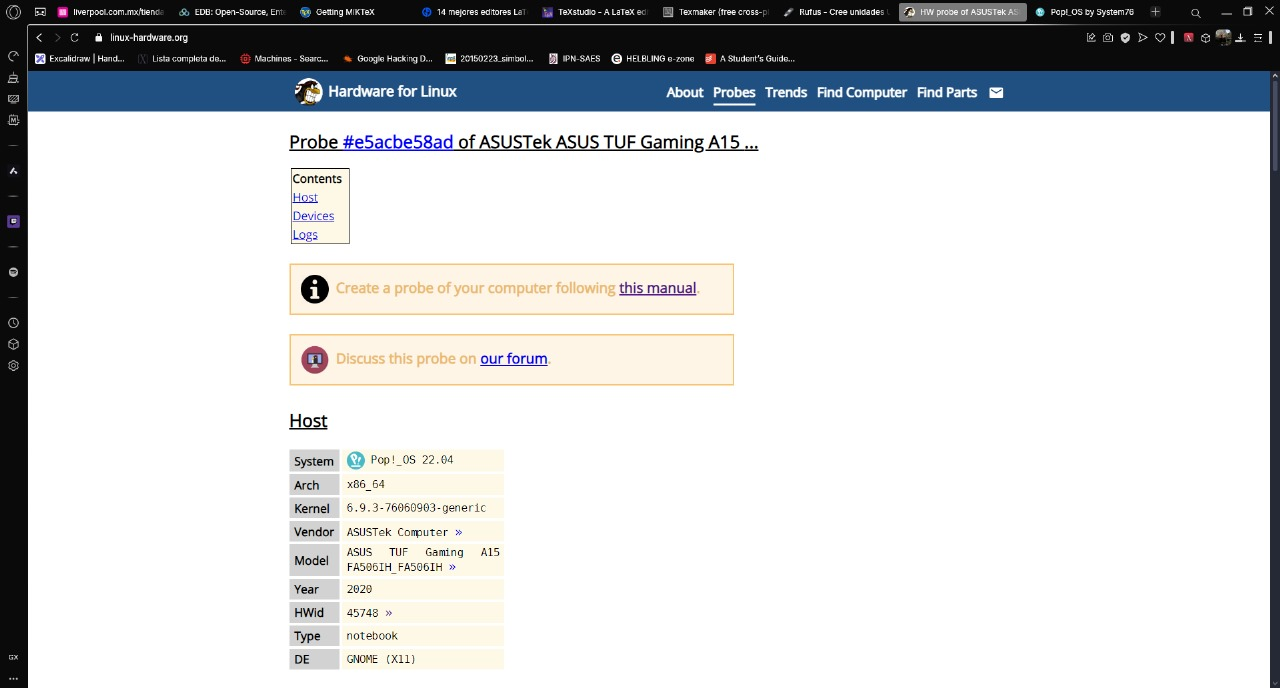
\includegraphics[width=0.95\textwidth]{./img/revision_linux-hardware.jpeg}
  \caption{Prueba en linux hardware}
\end{figure}

\clearpage

\subsection{Requerimientos de Pop OS}

\subsubsection{Requerimientos minimos}

\begin{itemize}
  \item \textbf{Procesador:} CPU de 64 bits
  \item \textbf{RAM:} 4GB
  \item \textbf{Almacenamiento:} 20GB
\end{itemize}

\\\\
Los requerimentos recomendados son de una RAM de 8GB y todo lo demas igual.

  \section{Preparacion del equipo}

\subsection{Respaldo de datos}

Mi equipo cuenta con dos espacios de almacenamiento un SSD de 258GB en el que tiene instalado el sistema operativo windows y un disco duro de 1TB, en este se instalara el sistema linux para ello realicé una revision de la informacion que contenia para ver si era relevante respaldarla o no la mayor parte de la informacion fue eliminada. 

Una vez revisada toda la información y seleccionada la que queria preservar en un disco duro externo relice la copia de los datos.

\subsection{Descarga de los prerequisitos}

\subsubsection{Instalación de la iso}
Nos dirgimos a la pagina de \href{https://pop.system76.com/}{Pop OS} y seleccionamos la iso que nos interese, en mi caso seleccioné la iso que viene con los drivers de NVIDIA pre-instalados.

\begin{figure}[h]
  \begin{center}
    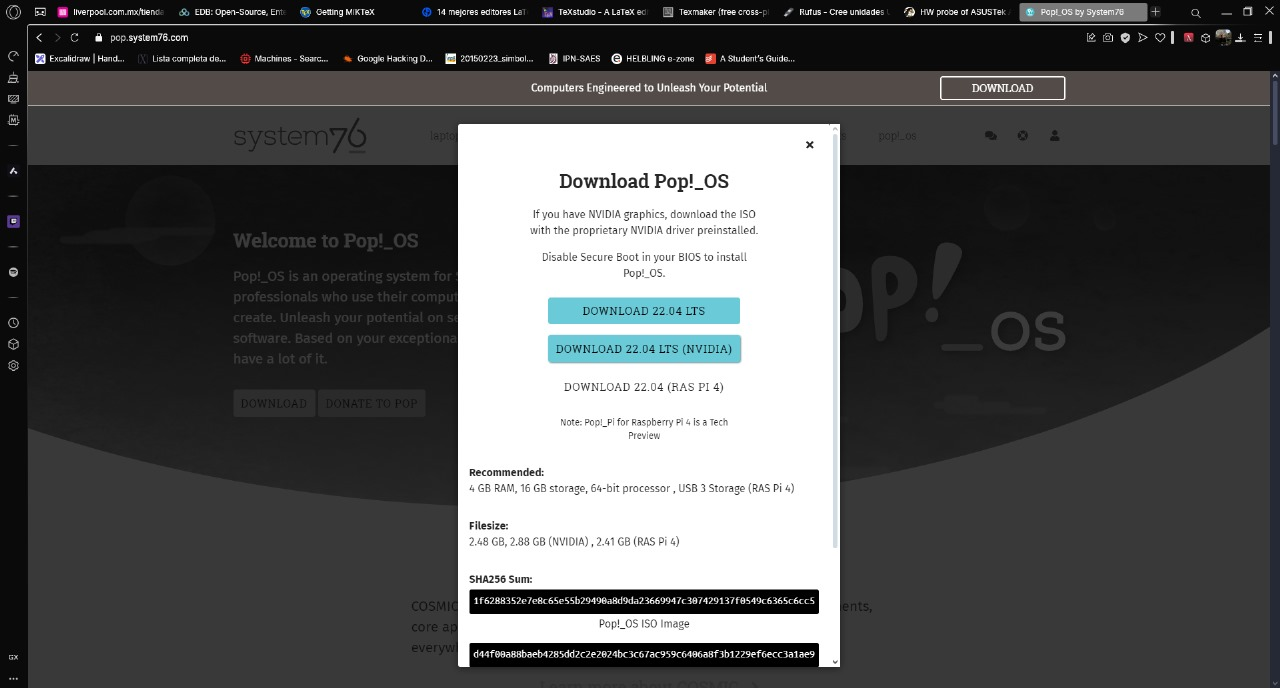
\includegraphics[width=0.95\textwidth]{img/download_popos.jpeg}
  \end{center}
  \caption{Descarga de la iso con drivers NVIDIA}\label{fig:download_popos}
\end{figure}

\clearpage
\subsubsection{Instalación de Rufus}

Una vez teniendo la iso procedemos a la instalacion de un programa para flashear una USB, para ello nos dirigimos a la pagina oficial de nuestro flasher \href{https://rufus.ie/es/}{Rufus} y descargamos el ejecutable.

Yo descaargue la versión portable para mayor comodidad. 

\begin{figure}[h]
  \begin{center}
    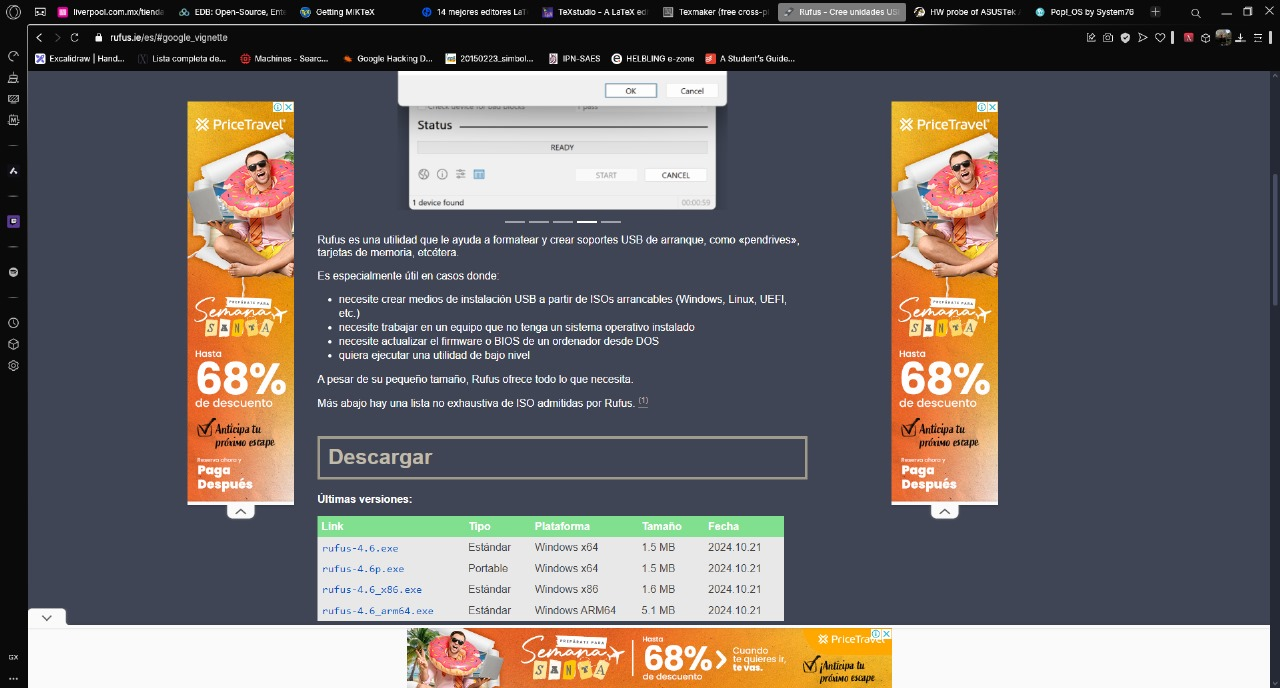
\includegraphics[width=0.75\textwidth]{img/download_rufus.jpeg}
  \end{center}
  \caption{Descarga de Rufus}\label{fig:download_rufus}
\end{figure}


\subsection{Flasheo de la USB}

Con la iso descargada y rufus listo procedemos a conectar la usb que usaremos para instalar nuestro sistema operativo.
\\\\
A continuación los pasos que seguí para la instalación
\begin{enumerate}
  \item Abrimos Rufus
  \item Seleccionamos la iso
  \item Seleccionamos el tipo de boot (UEFI/BIOS)
  \item Seleccionamos la USB
  \item Formateamos la USB y comienza la descompresion de la iso
\end{enumerate}

\begin{figure}[h]
  \begin{center}
    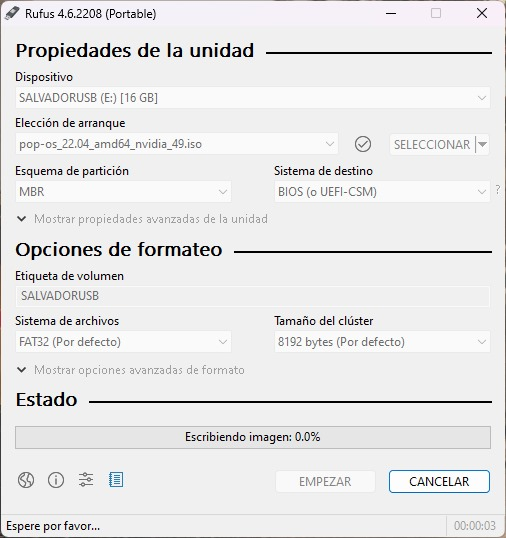
\includegraphics[width=0.3\textwidth]{img/usb_boot.jpeg}
  \end{center}
  \caption{Flasheo de USB}\label{fig:usb_boot}
\end{figure}

\\
Y esperamos que la instalacion finalice, esto puede llevar desde un par de minutos hasta una hora dependiendo del tamaño del sistema operativo.


\subsection{Instalación del sistema en el disco}

Con todo preparado podemos apagar la computadora y encenderla para entrar en el menú de arranque, en mi computadora se utiliza la tecla \keys{F2}; una vez en el menú se selecciona la USB booteable como método de arranque. 
\\
Con esto realizado se abrira la pantalla principal del sistema operativo(Vease \autoref{fig:pop_os_desktop})

\begin{figure}[h]
  \begin{center}
    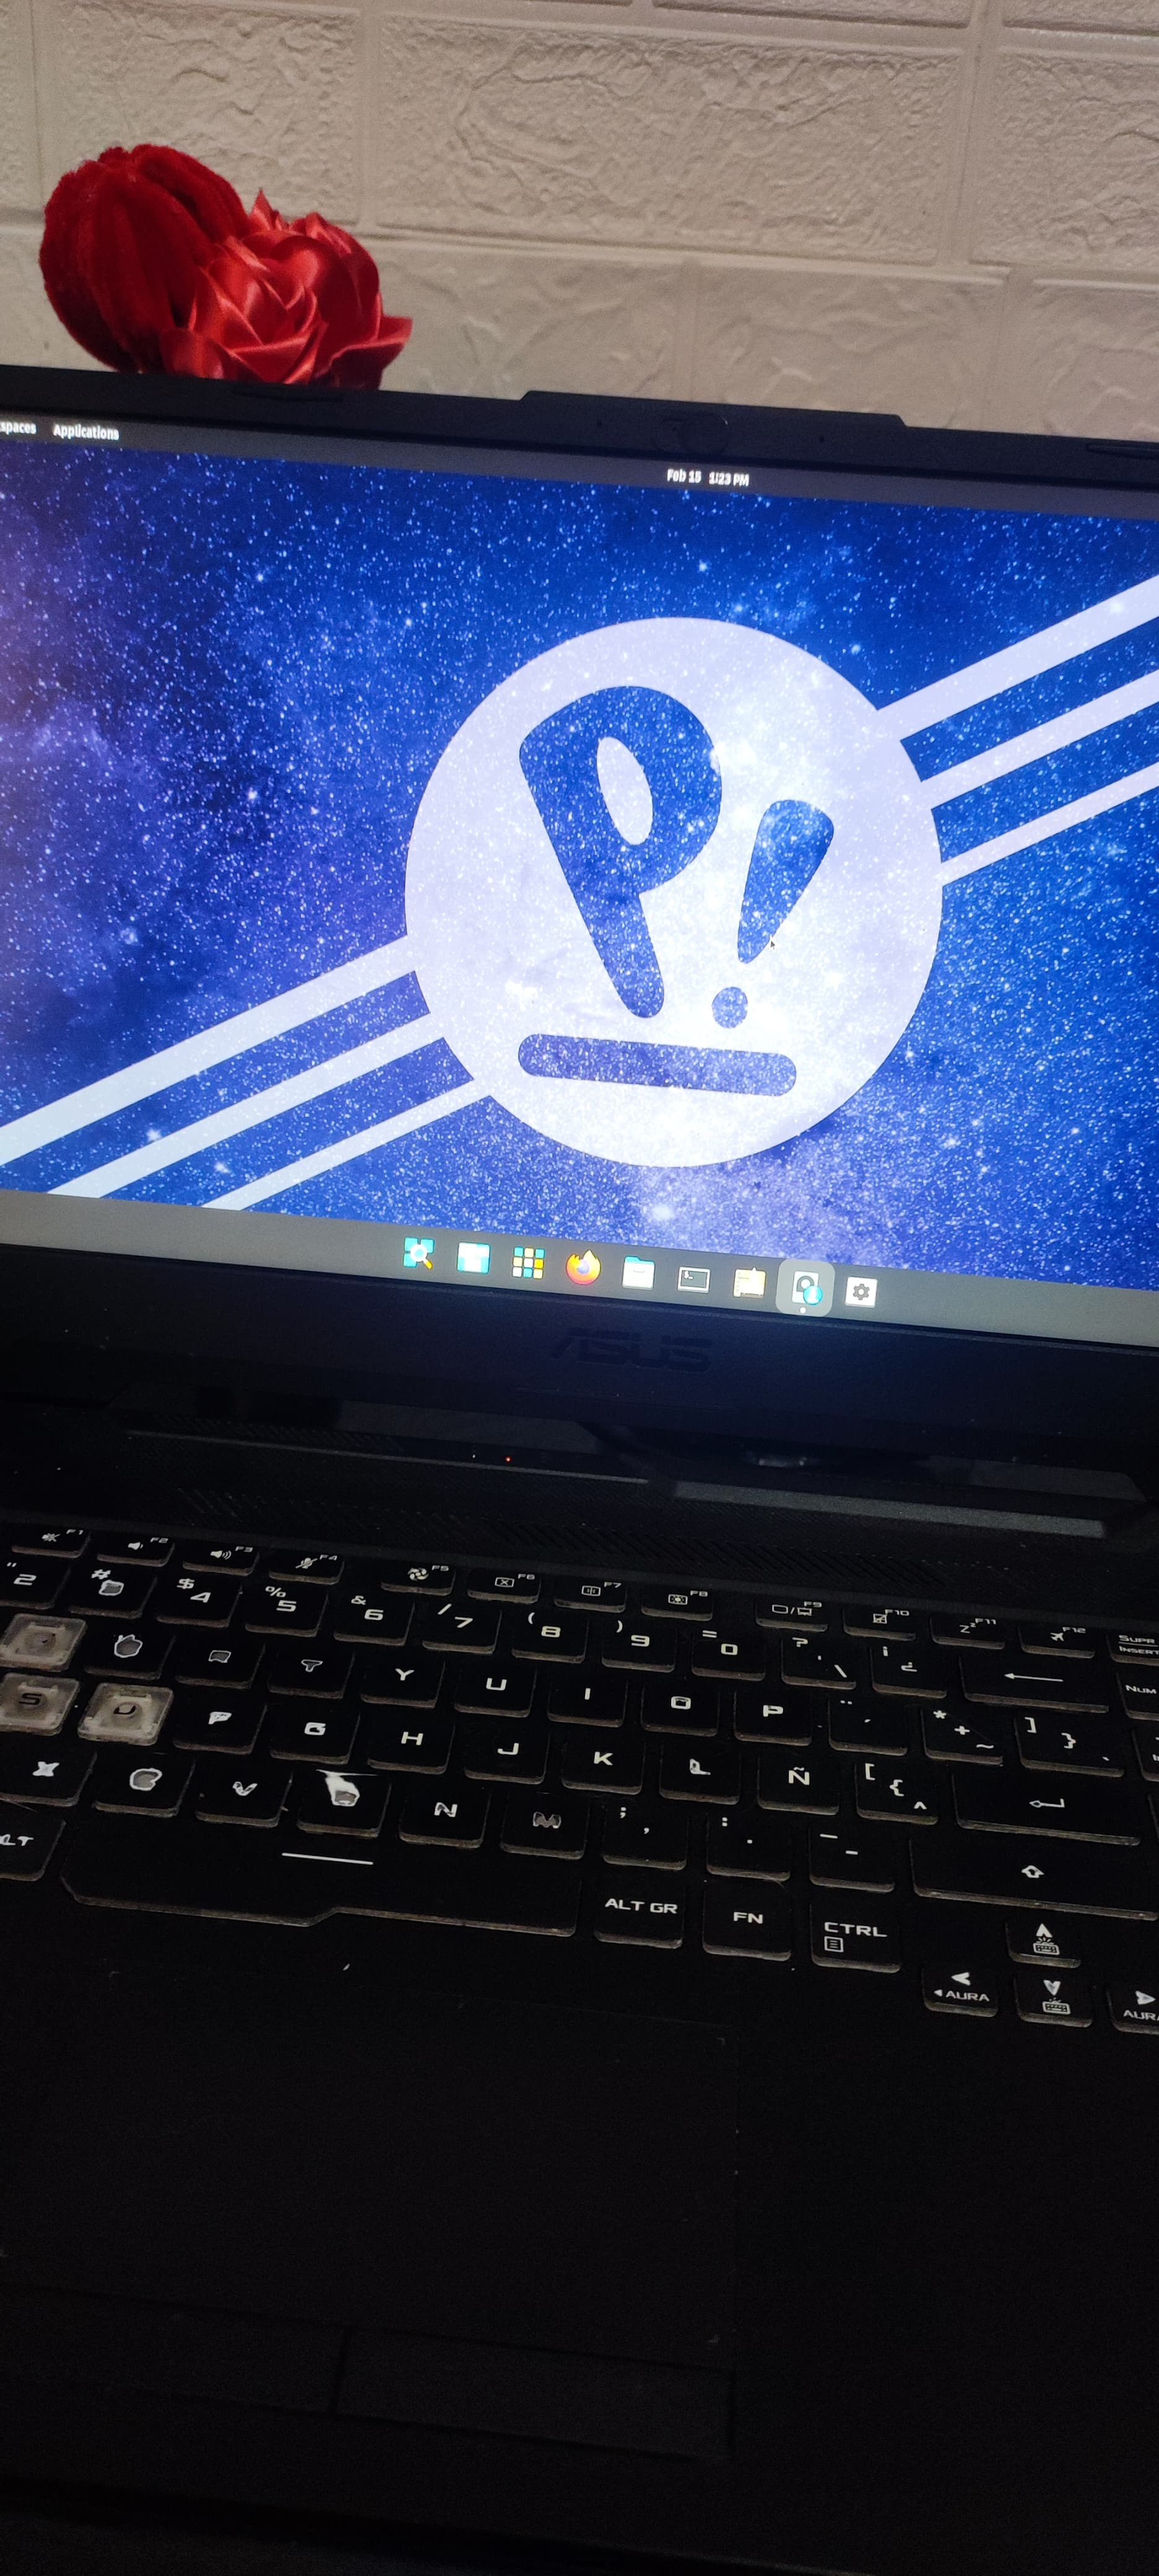
\includegraphics[width=0.25\textwidth]{img/pop_os_desktop.jpeg}
  \end{center}
  \caption{Escritorio de Pop OS}\label{fig:pop_os_desktop}
\end{figure}

Abrimos la aplicación de encargada de la instalación, seleccionamoos el idioma de la instalación y la distribucion de teclado apropiada. 
Una vez hecho esto procedemos a crear las particiones del sistema.

\begin{table}[h]
  \centering
  \begin{tabular}{ |p{3cm}|p{3cm}|p{3cm}|  }
    \hline
    \multicolumn{3}{|c|}{Configuración de particiones} \\
    \hline
    Partición & Tamaño & Sistema de archivos\\
    \hline
    EFI & 2.1 GB & FAT-32\\
    SWAP & 17GB & SWAP\\
    ROOT & 981GB & EXT4\\
    \hline
  \end{tabular}
  \label{tab:particiones}
  \caption{Tabla de particiones}
\end{table}

Dejamos que se limpie y se formateé el disco duro. 

\begin{figure}[h]
  \begin{center}
    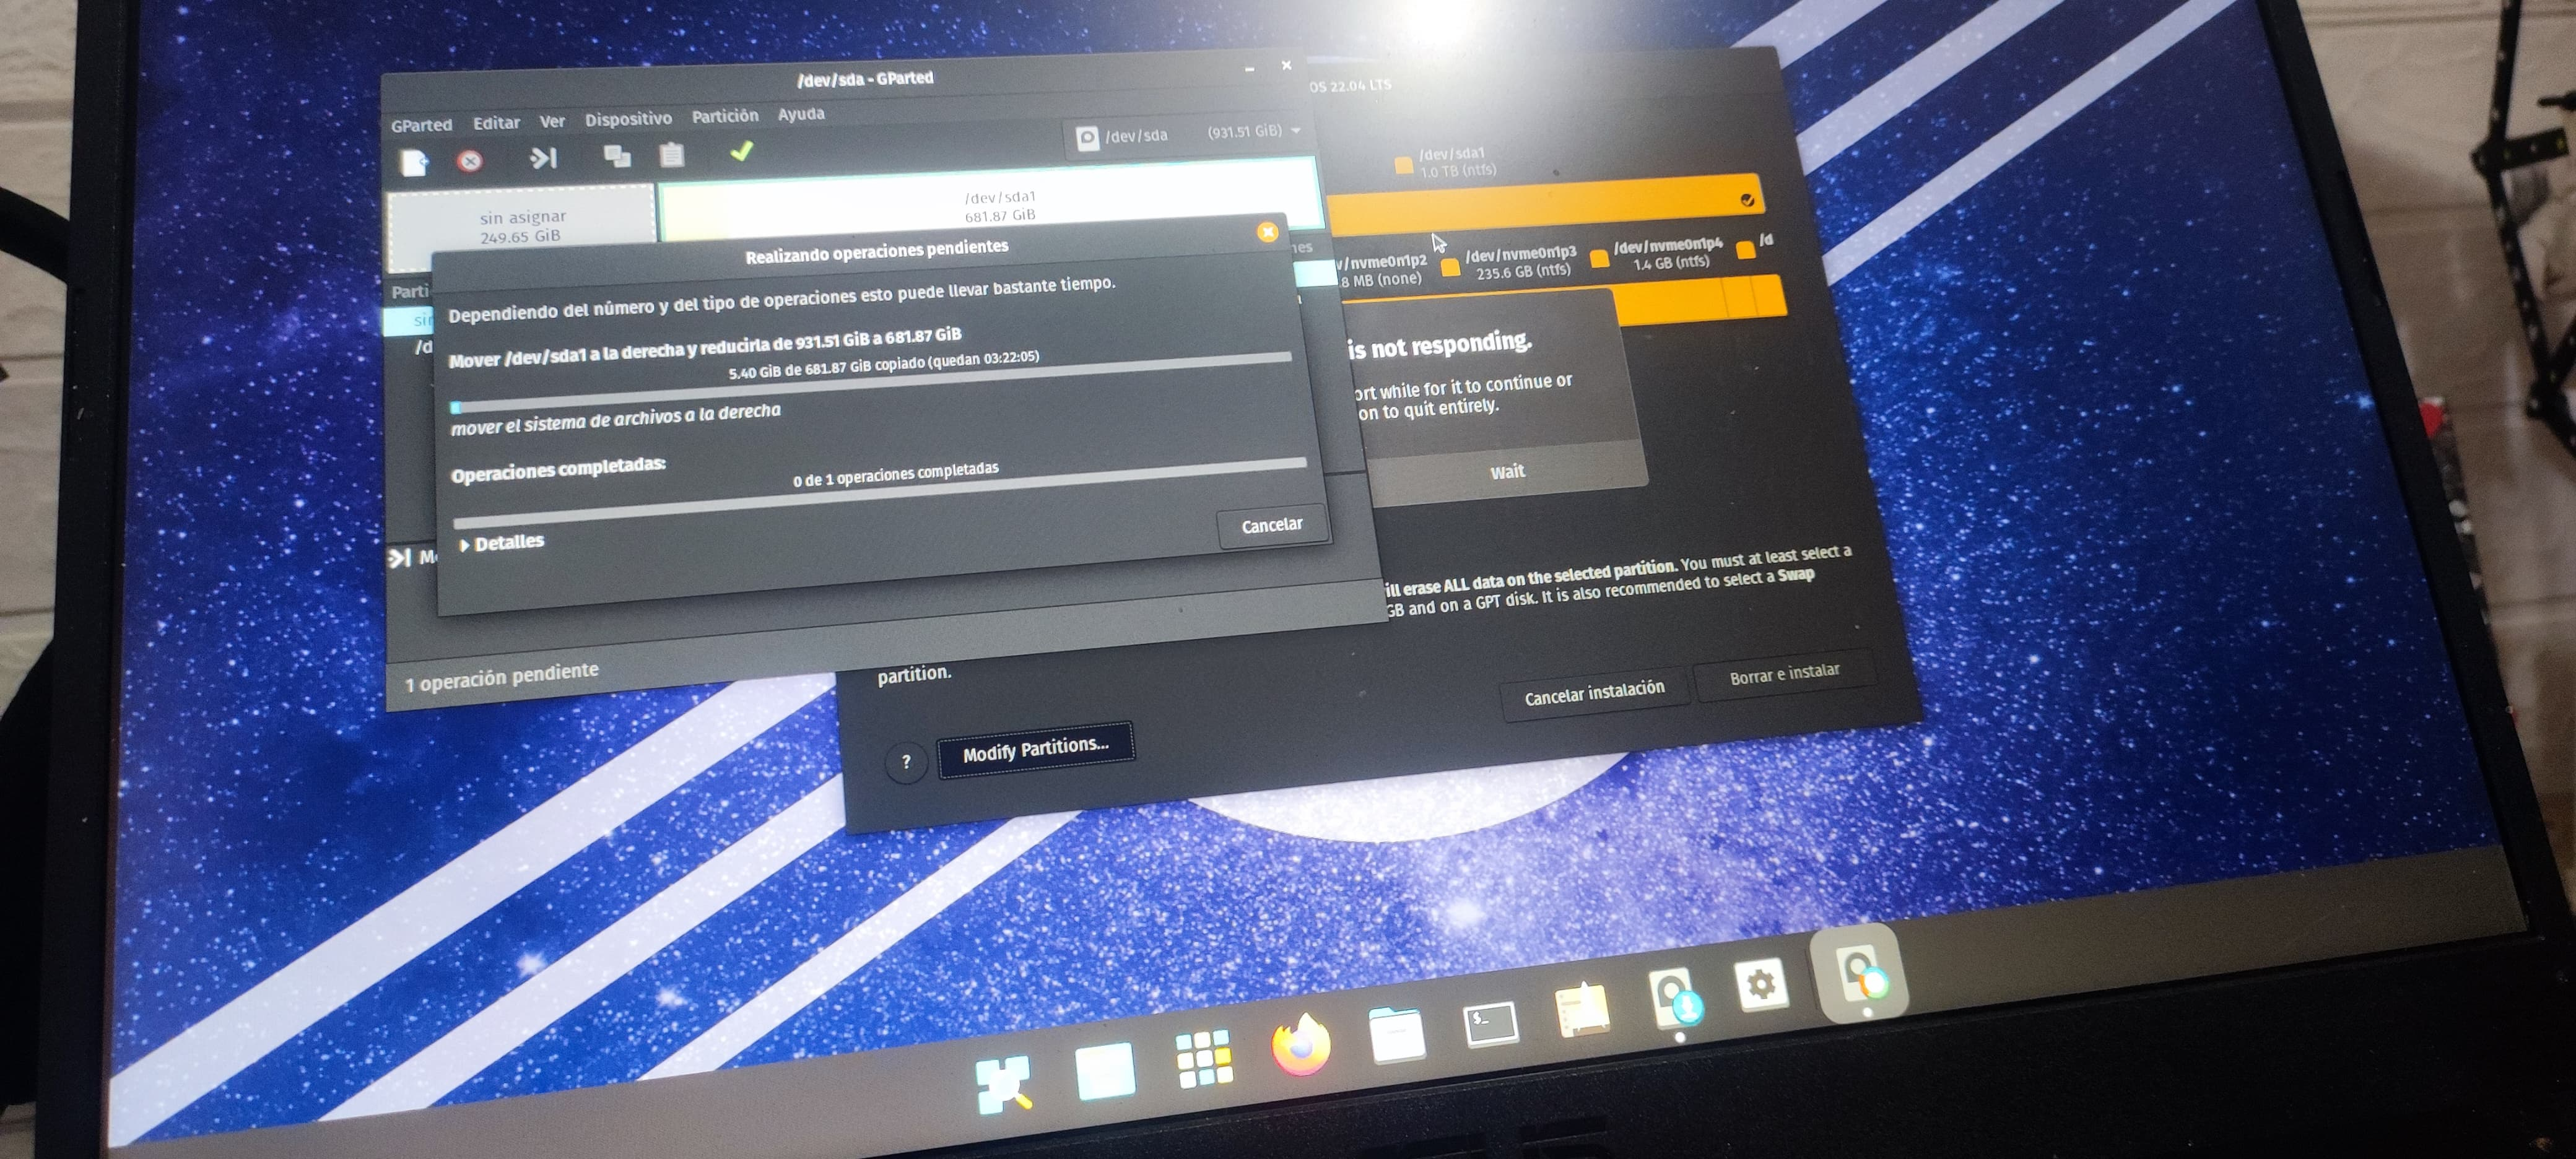
\includegraphics[width=0.3\textwidth]{img/particionado.jpeg}
  \end{center}
  \caption{Creando las particiones}\label{fig:particionado}
\end{figure}


Una ves formateado te pedira la creacion de un usuario y contraseña procedes con la instalacion y reinicias la computadora, cuando este reiniciando puedes quitar la usb y se iniciara directamente en el sistema operativo recien instalado. 

Inicias la sesión con el usuario que creaste anteriormente abres la terminal y aactualizas el sistema con los siguientes comandos:

\begin{lstlisting}[language=Bash]
  sudo apt update
  sudo apt upgrade
\end{lstlisting}


  \section{Conclusiones}

La instalación de Linux, específicamente Pop! OS, en la Asus TUF Gaming A15 fue un proceso bien estructurado y documentado. Se inició con una investigación previa para garantizar la compatibilidad del hardware, destacando que Pop! OS es una opción ideal debido a su optimización para tarjetas gráficas NVIDIA y su enfoque en la productividad.

La preparación del equipo incluyó el respaldo de datos y la descarga de los prerequisitos necesarios, como la imagen ISO del sistema y la herramienta Rufus para la creación de un USB booteable. Posteriormente, se realizó el flasheo de la USB y la instalación del sistema operativo, configurando correctamente las particiones del disco para un rendimiento óptimo.

En conclusión, el procedimiento seguido permitió una instalación exitosa y funcional de Pop! OS, asegurando estabilidad y rendimiento en la laptop. La documentación detallada de cada paso proporciona una guía útil para futuras instalaciones o referencias.

\end{document}
